\documentclass[11pt,a4paper]{article}
\usepackage[margin=20mm]{geometry}
\usepackage{amsmath,amssymb,booktabs,array,tikz,xcolor,fancyhdr,hyperref}
\usetikzlibrary{arrows.meta,positioning}
\definecolor{navy}{HTML}{16324F}
\definecolor{pale}{HTML}{EDF4FA}
\hypersetup{colorlinks=true,linkcolor=navy,urlcolor=navy}
\pagestyle{fancy}\fancyhf{}
\fancyhead[L]{\small\textcolor{navy}{Graph neural networks / Architecture guide}}
\fancyhead[R]{\small Configuration ranking}
\fancyfoot[R]{\small\thepage}
\setlength{\headheight}{14pt}
\setlength{\parindent}{0pt}\setlength{\parskip}{4pt}\raggedbottom
\renewcommand{\arraystretch}{1.18}
\newcommand{\code}[1]{\texttt{#1}}
\begin{document}
{\LARGE\bfseries\textcolor{navy}{GraphSAGE: explicit data flow}}\par
\textbf{Objective.} Choose which settings will make a computation run fastest.
The computation is a graph: nodes are operations and edges show their connections.
The same graph can run with different settings, such as memory layouts. The GNN
looks at each candidate's settings and the surrounding operations, gives it a score,
and ranks candidates from predicted fastest to slowest. Lower scores mean faster.

$B$ = candidates in one batch; $N$ = retained nodes. Blue boxes are processing
steps; green boxes hold data; dashed arrows supply graph information.

\begin{center}
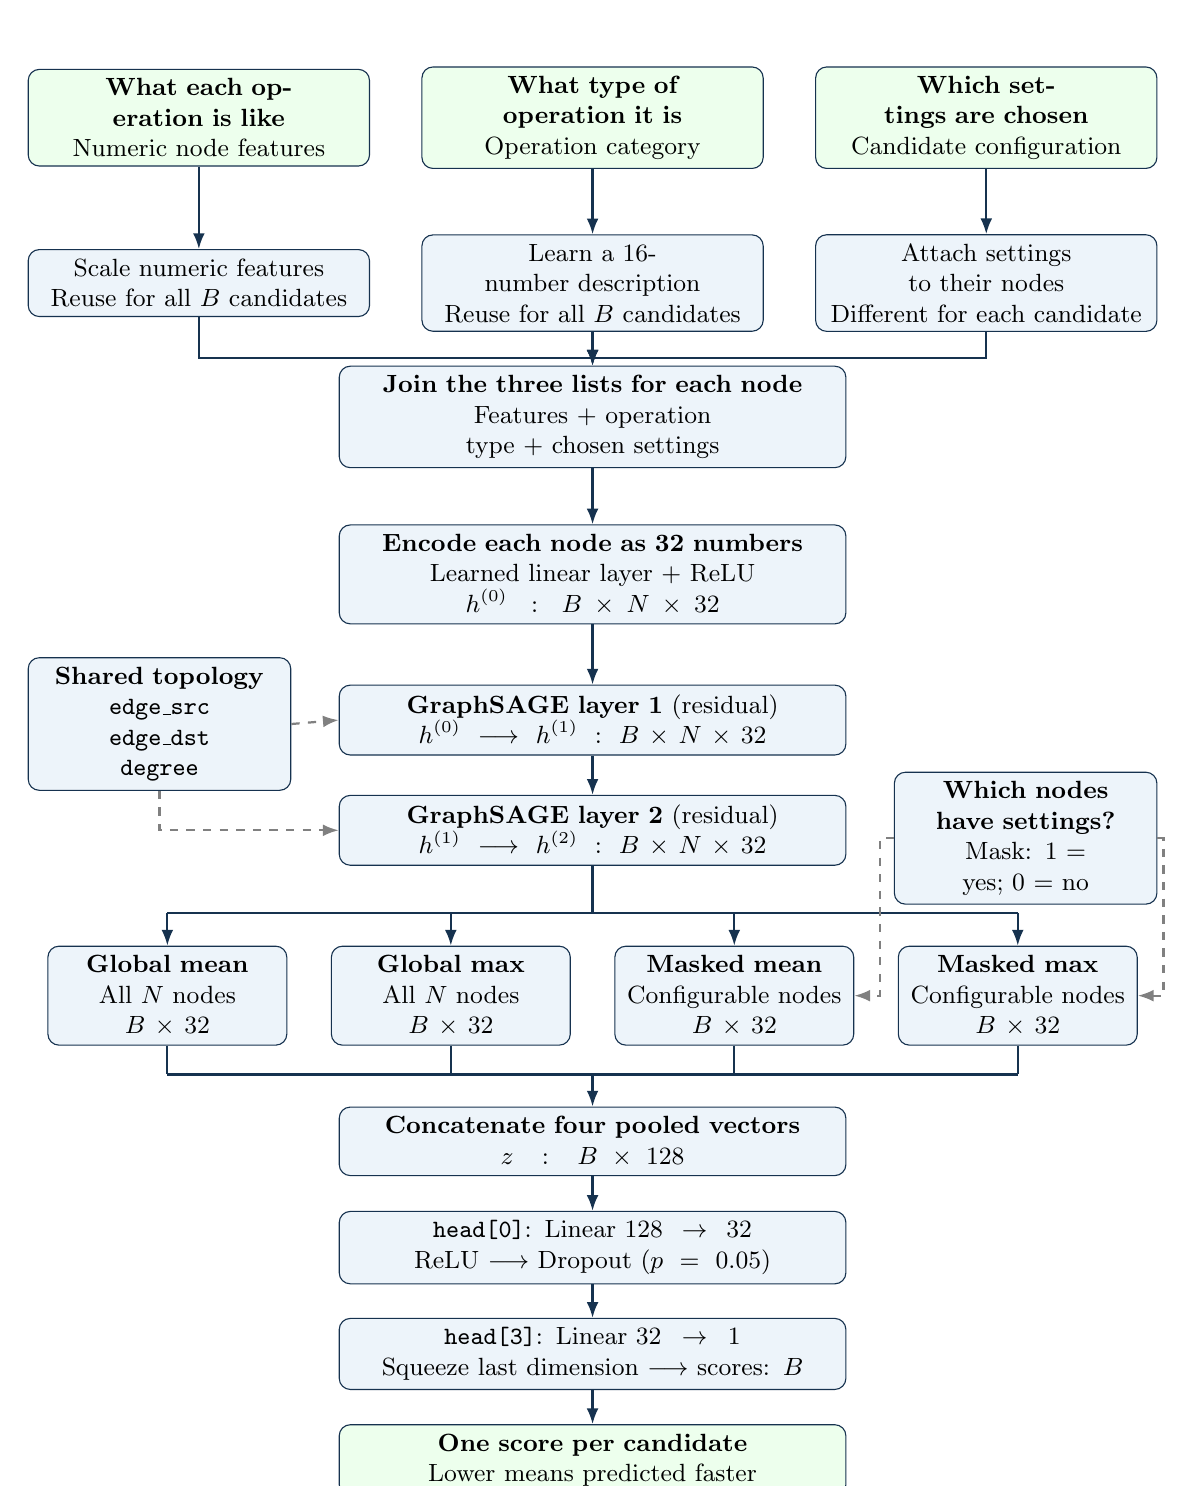
\begin{tikzpicture}[
 op/.style={draw=navy,fill=pale,rounded corners,align=center,text width=4.1cm,minimum height=0.85cm,font=\small},
 tensor/.style={op,fill=green!7!white},
 wide/.style={op,text width=6.2cm},
 pool/.style={op,text width=2.8cm,minimum height=0.95cm},
 arr/.style={-{Latex[length=2mm]},thick,draw=navy},
 meta/.style={arr,dashed,draw=gray},
 note/.style={font=\scriptsize,align=center,fill=white,inner sep=2pt}]
\node[tensor] (raw) at (-5,0) {\textbf{What each operation is like}\\Numeric node features};
\node[tensor] (opcode) at (0,0) {\textbf{What type of operation it is}\\Operation category};
\node[tensor] (config) at (5,0) {\textbf{Which settings are chosen}\\Candidate configuration};
\node[op] (base) at (-5,-2.1) {Scale numeric features\\Reuse for all $B$ candidates};
\node[op] (emb) at (0,-2.1) {Learn a 16-number description\\Reuse for all $B$ candidates};
\node[op] (conf) at (5,-2.1) {Attach settings to their nodes\\Different for each candidate};
\node[wide] (cat) at (0,-3.8) {\textbf{Join the three lists for each node}\\Features + operation type + chosen settings};
\node[wide] (proj) at (0,-5.8) {\textbf{Encode each node as 32 numbers}\\Learned linear layer + ReLU\\$h^{(0)}: B\times N\times32$};
\node[wide] (sage1) at (0,-7.65) {\textbf{GraphSAGE layer 1} (residual)\\$h^{(0)}\longrightarrow h^{(1)}: B\times N\times32$};
\node[wide] (sage2) at (0,-9.05) {\textbf{GraphSAGE layer 2} (residual)\\$h^{(1)}\longrightarrow h^{(2)}: B\times N\times32$};
\node[op,text width=3.1cm] (edges) at (-5.5,-7.7) {\textbf{Shared topology}\\\code{edge\_src}\\\code{edge\_dst}\\\code{degree}};
\node[op,text width=3.1cm] (mask) at (5.5,-9.15) {\textbf{Which nodes have settings?}\\Mask: 1 = yes; 0 = no};
\node[pool] (gm) at (-5.4,-11.15) {\textbf{Global mean}\\All $N$ nodes\\$B\times32$};
\node[pool] (gx) at (-1.8,-11.15) {\textbf{Global max}\\All $N$ nodes\\$B\times32$};
\node[pool] (cm) at (1.8,-11.15) {\textbf{Masked mean}\\Configurable nodes\\$B\times32$};
\node[pool] (cx) at (5.4,-11.15) {\textbf{Masked max}\\Configurable nodes\\$B\times32$};
\node[wide] (pooled) at (0,-13) {\textbf{Concatenate four pooled vectors}\\$z: B\times128$};
\node[wide] (head1) at (0,-14.35) {\code{head[0]}: Linear $128\to32$\\ReLU $\longrightarrow$ Dropout $(p=0.05)$};
\node[wide] (head2) at (0,-15.7) {\code{head[3]}: Linear $32\to1$\\Squeeze last dimension $\longrightarrow$ scores: $B$};
\node[tensor,text width=6.2cm] (scores) at (0,-17.05) {\textbf{One score per candidate}\\Lower means predicted faster};
\foreach \a/\b in {raw/base,opcode/emb,config/conf,emb/cat,cat/proj,proj/sage1,sage1/sage2,pooled/head1,head1/head2,head2/scores}
 \draw[arr] (\a)--(\b);
\draw[arr] (base.south)--(-5,-3.05)-|(cat.north);
\draw[arr] (conf.south)--(5,-3.05)-|(cat.north);
\draw[meta] (edges.east)--(sage1.west);
\draw[meta] (edges.south)|-(sage2.west);
\draw[thick,draw=navy] (sage2.south)--(0,-10.1);
\draw[thick,draw=navy] (-5.4,-10.1)--(5.4,-10.1);
\foreach \a in {gm,gx,cm,cx}\draw[arr] (\a.north |- 0,-10.1)--(\a.north);
\draw[meta] (mask.east)--(7.25,-9.15)--(7.25,-11.15)--(cx.east);
\draw[meta] (mask.west)--(3.65,-9.15)--(3.65,-11.15)--(cm.east);
\foreach \a in {gm,gx,cm,cx}\draw[thick,draw=navy] (\a.south)--(\a.south |- 0,-12.15);
\draw[thick,draw=navy] (-5.4,-12.15)--(5.4,-12.15);
\draw[arr] (0,-12.15)--(pooled.north);
\end{tikzpicture}
\end{center}
\small The two GraphSAGE blocks have separate learned weights. Their internal branches
are expanded after the terminology guide. Dropout is disabled for prediction.
\normalsize
\newpage
{\LARGE\bfseries\textcolor{navy}{The diagram in plain language}}\par
\subsection*{1. What does ``broadcast across $B$'' mean?}
$B$ is the number of candidate configurations processed together. For example,
with $B=3$, we evaluate three different settings for the \emph{same graph}.
The node features and operation types stay the same; the configuration features change.
\begin{center}
\begin{tabular}{@{}lll@{}}
\toprule
\textbf{Candidate} & \textbf{Shared information} & \textbf{Candidate-specific information}\\\midrule
1 & Same graph and operation types & Settings A\\
2 & Same graph and operation types & Settings B\\
3 & Same graph and operation types & Settings C\\\bottomrule
\end{tabular}
\end{center}
``Broadcast'' means making the shared information available for each candidate.
It does not create different graphs. In the code, this uses an expanded tensor view,
so broadcasting itself does not require physically copying that data $B$ times.
The figure calls this \textbf{reuse for all $B$ candidates}.

\subsection*{2. What does ``concatenate on the feature axis'' mean?}
It means \textbf{join each node's information into one longer list}. For example:
\[
\underbrace{[a,b,c]}_{\text{node features}}\quad
\underbrace{[d,e]}_{\text{configuration}}\quad
\underbrace{[f,g]}_{\text{operation embedding}}
\quad\longrightarrow\quad[a,b,c,d,e,f,g].
\]
The letters represent numbers. We join the lists belonging to the \emph{same node};
we do not merge different nodes. ``Feature axis'' is simply the dimension holding
this list. The figure calls this \textbf{join the three lists for each node}.

\subsection*{3. What is a configurable-node mask?}
Some operations have settings we can change. A mask marks those nodes with 1 and
other nodes with 0. Suppose only nodes B and D have configurable settings:
\[
\begin{array}{c|cccc}
\text{Node} & A & B & C & D\\\hline
\text{Mask} & 0 & 1 & 0 & 1
\end{array}
\]
The \textbf{masked mean and max} summarise B and D only. The \textbf{global mean and max}
summarise all nodes. This gives the model both overall context and a focused summary
of where settings can change. The mask identifies configurable locations; it does
not measure whether a particular value differs between two candidates.

\subsection*{4. Are two hops the two nearest neighbours?}
\textbf{Two hops means up to two connections away, not two selected neighbours.}
Starting from configurable node C:
\begin{center}
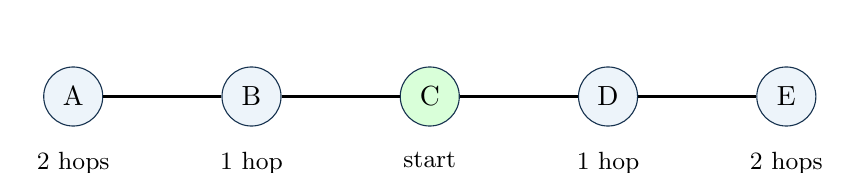
\begin{tikzpicture}[v/.style={circle,draw=navy,fill=pale,minimum size=0.75cm},node distance=1.5cm]
\node[v] (a) {A};\node[v,right=of a] (b) {B};
\node[v,right=of b,fill=green!15] (c) {C};
\node[v,right=of c] (d) {D};\node[v,right=of d] (e) {E};
\draw[thick] (a)--(b)--(c)--(d)--(e);
\node[below=0.2cm of a,font=\small] {2 hops};
\node[below=0.2cm of b,font=\small] {1 hop};
\node[below=0.2cm of c,font=\small] {start};
\node[below=0.2cm of d,font=\small] {1 hop};
\node[below=0.2cm of e,font=\small] {2 hops};
\end{tikzpicture}
\end{center}
If C has 20 directly connected neighbours, all 20 are one hop away.
This design first selects a neighbourhood within two hops of configurable nodes
(subject to its size target). It then applies two message-passing layers, allowing
information to travel up to two connections within that retained graph.
\newpage
{\LARGE\bfseries\textcolor{navy}{Inside each GraphSAGE block}}\par
Each layer collects information from \textbf{direct neighbours (1 hop)}.
\textbf{Repeat twice to capture information up to 2 hops away} within the retained graph.

\begin{center}
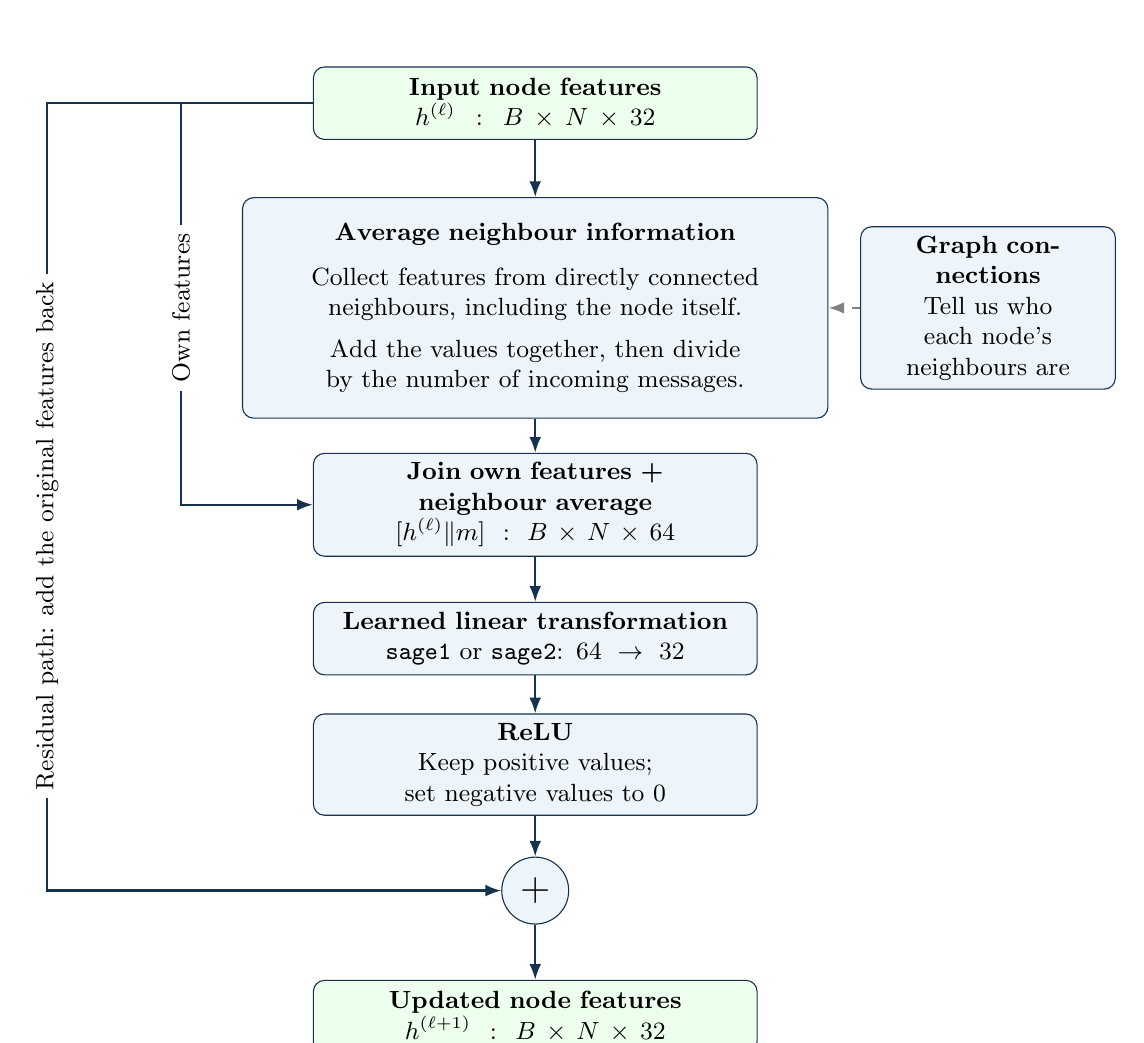
\begin{tikzpicture}[
 op/.style={draw=navy,fill=pale,rounded corners,align=center,text width=5.4cm,minimum height=0.92cm,font=\small},
 tensor/.style={op,fill=green!7!white},
 arr/.style={-{Latex[length=2mm]},thick,draw=navy},
 meta/.style={arr,dashed,draw=gray},
 lab/.style={font=\small,fill=white,align=center,inner sep=3pt}]
\node[tensor] (h) at (0,0) {\textbf{Input node features}\\$h^{(\ell)}: B\times N\times32$};
\node[op,text width=7.2cm,minimum height=2.8cm] (average) at (0,-2.6) {\textbf{Average neighbour information}\\[5pt]
Collect features from directly connected\\neighbours, including the node itself.\\[4pt]
Add the values together, then divide\\by the number of incoming messages.};
\node[op,text width=3cm] (graph) at (5.75,-2.6) {\textbf{Graph connections}\\Tell us who each node's neighbours are};
\node[op] (cat) at (0,-5.1) {\textbf{Join own features + neighbour average}\\$[h^{(\ell)}\Vert m]: B\times N\times64$};
\node[op] (linear) at (0,-6.8) {\textbf{Learned linear transformation}\\\code{sage1} or \code{sage2}: $64\to32$};
\node[op] (relu) at (0,-8.4) {\textbf{ReLU}\\Keep positive values; set negative values to 0};
\node[draw=navy,fill=pale,circle,minimum size=0.85cm,font=\Large] (plus) at (0,-10) {$+$};
\node[tensor] (out) at (0,-11.6) {\textbf{Updated node features}\\$h^{(\ell+1)}: B\times N\times32$};
\foreach \a/\b in {h/average,average/cat,cat/linear,linear/relu,relu/plus,plus/out}\draw[arr] (\a)--(\b);
\draw[meta] (graph.west)--(average.east);
\draw[arr] (h.west)--(-4.5,0)--(-4.5,-5.1)--(cat.west);
\node[lab,rotate=90] at (-4.5,-2.6) {Own features};
\draw[arr] (h.west)--(-6.2,0)--(-6.2,-10)--(plus.west);
\node[lab,rotate=90] at (-6.2,-5.5) {Residual path: add the original features back};
\end{tikzpicture}
\end{center}
\textbf{Topology preparation before either layer:}
\begin{center}
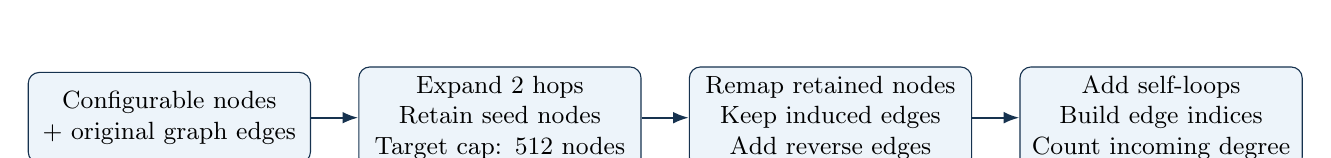
\begin{tikzpicture}[box/.style={draw=navy,fill=pale,rounded corners,text width=3.35cm,align=center,font=\small,minimum height=1.15cm},arr/.style={-{Latex[length=2mm]},thick,draw=navy},node distance=0.6cm]
\node[box] (a) {Configurable nodes\\+ original graph edges};
\node[box,right=of a] (b) {Expand 2 hops\\Retain seed nodes\\Target cap: 512 nodes};
\node[box,right=of b] (c) {Remap retained nodes\\Keep induced edges\\Add reverse edges};
\node[box,right=of c] (d) {Add self-loops\\Build edge indices\\Count incoming degree};
\foreach \x/\y in {a/b,b/c,c/d}\draw[arr] (\x)--(\y);
\end{tikzpicture}
\end{center}
\small $E$ counts entries in the prepared edge list, including duplicates and self-loops.
Self-loops make each node contribute to its own neighbour mean as well as the explicit
self-feature and residual paths. If the seed set exceeds 512 nodes, all seeds are kept.
\normalsize
\newpage
{\LARGE\bfseries\textcolor{navy}{Why this design works this way}}\par
\textbf{The question:} given the same computation graph, which configuration should
run faster? A node represents an operation, an edge connects operations, and a
configuration specifies choices such as memory layouts at selected nodes.

\begin{center}
\begin{tabular}{@{}>{\raggedright\arraybackslash}p{4.3cm}>{\raggedright\arraybackslash}p{10.7cm}@{}}
\toprule
\textbf{Design choice} & \textbf{Reasoning}\\\midrule
Inject configuration features & The graph stays the same across candidates. Attaching candidate-specific settings to nodes lets their scores differ.\\[4pt]
Embed operation types & A learned 16-D vector represents each operation category without treating its integer ID as a numerical magnitude.\\[4pt]
Use a local subgraph & Start from configurable nodes and retain nearby context. This reduces computation but can omit useful distant information.\\[4pt]
Pass messages twice & A node combines its own features with nearby operations. Two rounds allow information to travel up to two prepared edges.\\[4pt]
Keep residual paths & Add the previous node representation back after each update, preserving a direct path for information and gradients.\\[4pt]
Pool globally and locally & Whole-graph summaries capture broader context; configurable-node summaries keep attention on where settings change. Mean captures average patterns; max captures strong activations.\\[4pt]
Learn a scalar ranking score & Comparing candidates requires their relative order. Predicting runtime in seconds is not necessary for that purpose.\\\bottomrule
\end{tabular}
\end{center}

\subsection*{How the model learns}
Training compares candidate configurations of the \emph{same} graph using their
measured runtimes. If configuration $f$ is faster than configuration $s$, the
network should output $s_f<s_s$.
\begin{center}
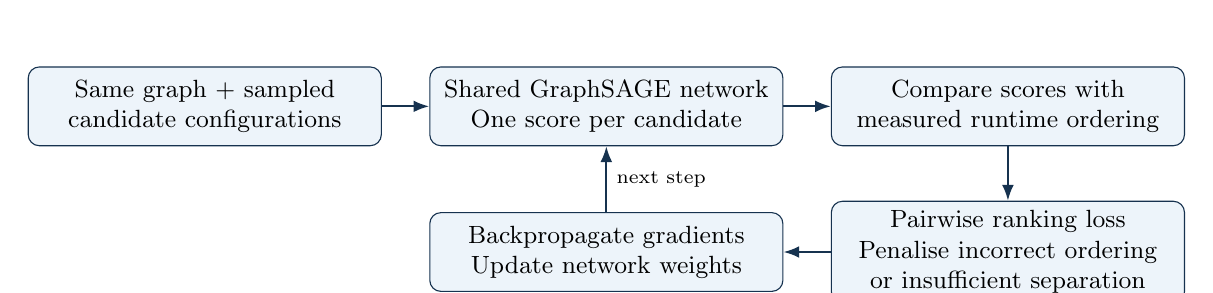
\begin{tikzpicture}[box/.style={draw=navy,fill=pale,rounded corners,text width=4.25cm,align=center,font=\small,minimum height=1cm},arr/.style={-{Latex[length=2mm]},thick,draw=navy}]
\node[box] (a) at (0,0) {Same graph + sampled\\candidate configurations};
\node[box] (b) at (5.1,0) {Shared GraphSAGE network\\One score per candidate};
\node[box] (c) at (10.2,0) {Compare scores with\\measured runtime ordering};
\node[box] (d) at (10.2,-1.85) {Pairwise ranking loss\\Penalise incorrect ordering\\or insufficient separation};
\node[box] (e) at (5.1,-1.85) {Backpropagate gradients\\Update network weights};
\foreach \x/\y in {a/b,b/c,c/d,d/e}\draw[arr] (\x)--(\y);
\draw[arr] (e.north)--node[right,font=\scriptsize]{next step}(b.south);
\end{tikzpicture}
\end{center}
For a faster/slower pair, a margin loss is
\[
\mathcal{L}_{f,s}=\max(0,m+s_f-s_s),\qquad m>0.
\]
With margin $m=0.1$, scores $s_f=0.2$, $s_s=0.5$ incur zero loss. Reversing them
incurs $0.4$. Average over eligible pairs; near-equal runtimes may be excluded
to avoid learning from tiny differences. In this implementation, a batch with
no eligible pairs falls back to a regression loss on centred log runtimes.

\subsection*{How the trained model is used}
Keep the graph fixed, score each candidate in batches, then sort candidates by
score in ascending order. Measured runtimes are needed for training and evaluation,
not for predicting new candidate rankings. Dropout is disabled for prediction.

\textbf{Design choices.} Width 32, two layers and the 512-node target belong to this
example; they are not requirements of GraphSAGE. Scores are not runtimes in seconds.
\end{document}
